\documentclass[conference]{IEEEtran}
\IEEEoverridecommandlockouts
\usepackage{cite}
\usepackage{amsmath,amssymb,amsfonts,amsthm}
\usepackage{algorithmic}
\usepackage{algorithm}
\usepackage{graphicx}
\usepackage{textcomp}
\usepackage{xcolor}
\usepackage{booktabs}
\usepackage{multirow}
\usepackage{tikz}
\usetikzlibrary{patterns,arrows.meta,positioning,calc}

\newtheorem{theorem}{Theorem}
\newtheorem{lemma}[theorem]{Lemma}
\newtheorem{definition}{Definition}

\def\BibTeX{{\rm B\kern-.05em{\sc i\kern-.025em b}\kern-.08em
    T\kern-.1667em\lower.7ex\hbox{E}\kern-.125emX}}

\begin{document}

\title{Dynamic Platoon Formation of Multi-Type Autonomous Vehicles for Sustainable Urban Mobility}

\author{
\IEEEauthorblockN{Jaeyun Ree}
\IEEEauthorblockA{
\textit{Faculty of Information Technology} \\
\textit{Monash University} \\
Melbourne, VIC, Australia \\
jree0010@student.monash.edu
}
\and
\IEEEauthorblockN{Mohammed Eunus Ali}
\IEEEauthorblockA{
\textit{Faculty of Information Technology} \\
\textit{Monash University} \\
Melbourne, VIC, Australia \\
eunus.ali@monash.edu
}
}

\maketitle

\begin{abstract}
This paper addresses the energy inefficiency of single-occupancy vehicles by introducing a novel cooperative autonomous vehicle system where smaller Passive Vehicles (PVs) can be physically towed by larger Active Vehicles (AVs) during shared highway segments. Unlike traditional platooning that relies solely on aerodynamic drafting, our approach enables near-complete energy elimination for towed vehicles. We formulate the platoon formation problem as a constrained optimization problem on a one-dimensional highway model and propose two algorithms: a Greedy Maximum-Weight Matching algorithm that provides computational efficiency with $O(NM\log(NM))$ complexity, and an Enhanced Hungarian Algorithm that guarantees optimal solutions with $O((N+M)^3)$ complexity. A key innovation is the multi-segment matching capability, allowing a single PV to be towed by multiple AVs across different route segments. Experimental evaluation on synthetic highway scenarios demonstrates that both algorithms achieve significant energy savings, with the Hungarian algorithm consistently finding optimal solutions while the Greedy approach provides near-optimal results (within 3\% of optimal) at substantially lower computational cost.
\end{abstract}

\begin{IEEEkeywords}
autonomous vehicles, vehicle platooning, energy efficiency, Hungarian algorithm, combinatorial optimization, intelligent transportation systems
\end{IEEEkeywords}

%==============================================================================
% SECTION 1: INTRODUCTION
%==============================================================================
\section{Introduction}

% Paragraph 1: High-level motivation (world problem + statistics)
The persistent over-reliance on single-occupancy vehicles poses significant challenges to urban transportation sustainability. According to the U.S. Department of Transportation, single-occupancy vehicles account for approximately 76\% of commuter trips, contributing substantially to traffic congestion, energy consumption, and carbon emissions~\cite{usdot2023}. The transportation sector alone is responsible for nearly 29\% of total greenhouse gas emissions in the United States, with light-duty vehicles contributing the largest share~\cite{epa2023}. This inefficiency is particularly pronounced along shared routes where multiple individuals travel similar paths yet operate their vehicles independently.

% Paragraph 2: Problem and idea (platooning/cooperation concept)
Autonomous vehicle (AV) technology presents a transformative opportunity to address these challenges through coordinated vehicle operation. This paper introduces a novel concept of \textit{active} and \textit{passive} autonomous vehicles, where smaller Passive Vehicles (PVs) can temporarily attach to larger Active Vehicles (AVs) during shared highway segments. Unlike traditional vehicle platooning that maintains physical separation between vehicles, our approach enables physical coupling where a PV's propulsion system is deactivated while being towed, leading to energy savings that approach 100\% for the towed vehicle during the attached phase. This paradigm shifts transportation from isolated driving to an on-demand, energy-transfer-based mobility service.

% Paragraph 3: Related work sketch and differentiation
Existing research on cooperative vehicle systems spans several related but distinct areas. Traditional platooning systems~\cite{tsugawa2016review,bergenhem2012overview} focus on coordinated driving with aerodynamic benefits, typically achieving 10-20\% fuel savings through drafting. Ridesharing and carpooling optimization~\cite{furuhata2013ridesharing,agatz2012optimization} address passenger matching but not vehicle coupling. Eco-driving strategies~\cite{sciarretta2015optimal,hellstrom2009look} optimize individual vehicle behavior without inter-vehicle coordination. The assignment problem we address relates to the classic bipartite matching literature~\cite{kuhn1955hungarian,munkres1957algorithms}, though our multi-segment matching with capacity constraints introduces novel complexity. While these approaches offer incremental improvements, they do not address the fundamental inefficiency of independent propulsion for vehicles with overlapping routes.

% Paragraph 4: Our solution summary (big picture)
We formulate the platoon formation problem on a one-dimensional highway model where the objective is to maximize total energy savings through strategic PV-to-AV assignments. To solve this problem, we propose two complementary algorithms. The \textit{Greedy Maximum-Weight Matching} algorithm provides computational efficiency suitable for real-time applications, while the \textit{Enhanced Hungarian Algorithm} guarantees optimal solutions for scenarios where optimality is paramount. A key innovation is our multi-segment matching capability: rather than restricting each PV to a single AV, our algorithms allow a PV to be towed by different AVs across different segments of its route, significantly improving overall system efficiency.

% Paragraph 5: Contributions (what we show in results)
The main contributions of this paper are:
\begin{itemize}
    \item A formal one-dimensional problem formulation that captures the essential trade-offs in cooperative vehicle platooning, with precise mathematical notation and constraint specification.
    \item A Greedy algorithm with $O(NM\log(NM))$ complexity that achieves provable $\frac{1}{2}$-approximation through iterative maximum-weight matching.
    \item An Enhanced Hungarian algorithm with capacity constraints that guarantees optimal assignments with $O((N+M)^3)$ complexity per iteration.
    \item Multi-segment matching capability allowing PVs to be towed by multiple AVs across their routes, with point-wise capacity tracking.
    \item Comprehensive experimental evaluation demonstrating algorithm performance across varying capacity configurations, highway lengths, and vehicle densities.
\end{itemize}

%==============================================================================
% SECTION 2: PROBLEM DEFINITION
%==============================================================================
\section{Problem Formulation}

We formalize the platoon formation problem on a simplified one-dimensional highway model. This abstraction captures the essential optimization trade-offs while enabling tractable analysis. Extension to general road networks is discussed in Section~\ref{sec:conclusion}.

\subsection{Notation Summary}

Table~\ref{tab:notation} summarizes the key notation used throughout this paper.

\begin{table}[htbp]
\caption{Summary of Notation}
\label{tab:notation}
\centering
\begin{tabular}{cl}
\toprule
\textbf{Symbol} & \textbf{Description} \\
\midrule
$L$ & Highway length \\
$\mathcal{A}$ & Set of Active Vehicles (AVs), $|\mathcal{A}| = N$ \\
$\mathcal{P}$ & Set of Passive Vehicles (PVs), $|\mathcal{P}| = M$ \\
$e_i^a, x_i^a$ & Entry and exit points of AV $a_i$ \\
$e_j^p, x_j^p$ & Entry and exit points of PV $p_j$ \\
$C_i$ & Towing capacity of AV $a_i$ \\
$t_i^a, v_i^a$ & Entry time and speed of AV $a_i$ \\
$d_{ij}$ & Shared travel distance between $a_i$ and $p_j$ \\
$S_{ij}$ & Energy saving when $p_j$ is towed by $a_i$ \\
$cp_{ij}, dp_{ij}$ & Coupling and decoupling points \\
$L_{min}$ & Minimum shared distance for platooning \\
$\tau$ & Time tolerance for coupling synchronization \\
\bottomrule
\end{tabular}
\end{table}

\subsection{System Model}

We consider a coordinated platoon formation system operating on a unidirectional highway segment of length $L$. The system comprises two distinct vehicle classes.

\begin{definition}[Active Vehicle]
An Active Vehicle (AV) $a_i \in \mathcal{A}$ is a larger autonomous vehicle capable of towing multiple smaller vehicles. Each AV is characterized by the tuple $(e_i^a, x_i^a, C_i, t_i^a, v_i^a)$ where $e_i^a, x_i^a \in [0, L]$ are entry and exit points, $C_i \in \mathbb{Z}^+$ is the towing capacity, and $t_i^a, v_i^a$ are the entry time and constant speed.
\end{definition}

\begin{definition}[Passive Vehicle]
A Passive Vehicle (PV) $p_j \in \mathcal{P}$ is a smaller autonomous vehicle that can be towed by AVs. Each PV is characterized by the tuple $(e_j^p, x_j^p, t_j^p, v_j^p)$ where $e_j^p, x_j^p \in [0, L]$ are entry and exit points, and $t_j^p, v_j^p$ are entry time and self-driving speed.
\end{definition}

\subsection{Shared Path and Energy Model}

For an AV $a_i$ and PV $p_j$, the \textit{shared path} is the overlap of their routes:
\begin{equation}
    d_{ij} = \max(0, \min(x_i^a, x_j^p) - \max(e_i^a, e_j^p))
    \label{eq:shared}
\end{equation}

The coupling point $cp_{ij}$ (where PV attaches) and decoupling point $dp_{ij}$ (where PV detaches) are:
\begin{align}
    cp_{ij} &= \max(e_i^a, e_j^p) \label{eq:cp}\\
    dp_{ij} &= \min(x_i^a, x_j^p) \label{eq:dp}
\end{align}

The energy saving $S_{ij}$ when PV $p_j$ is towed by AV $a_i$ is proportional to the shared distance:
\begin{equation}
    S_{ij} = \alpha \cdot d_{ij}
    \label{eq:saving}
\end{equation}
where $\alpha$ is an energy coefficient. For simplicity, we set $\alpha = 1$, making energy saving equivalent to distance saved.

\subsection{Multi-Segment Matching}

A key innovation of our formulation is \textit{multi-segment matching}: a single PV can be matched to multiple AVs across different segments of its route.

\begin{definition}[Segment Assignment]
A segment assignment for PV $p_j$ to AV $a_i$ is a tuple $(p_j, a_i, s, e)$ where $[s, e] \subseteq [e_j^p, x_j^p]$ is the segment during which $p_j$ is towed by $a_i$.
\end{definition}

For PV $p_j$, its route from $e_j^p$ to $x_j^p$ can be partitioned into segments, where each segment is either:
\begin{itemize}
    \item \textit{Covered}: PV is towed by an AV (energy saved)
    \item \textit{Uncovered}: PV drives independently (no energy saved)
\end{itemize}

\subsection{Optimization Problem}

Let $x_{ij}^{(k)} \in \{0, 1\}$ be a binary decision variable indicating whether PV $p_j$ is assigned to AV $a_i$ for segment $k$. The optimization problem is:

\begin{align}
    \max \quad & \sum_{i=1}^{N} \sum_{j=1}^{M} \sum_{k} x_{ij}^{(k)} \cdot S_{ij}^{(k)} \label{eq:obj}\\
    \text{s.t.} \quad & \sum_{j: point \in [cp_{ij}, dp_{ij}]} x_{ij}^{(k)} \leq C_i \quad \forall i, \forall point \label{eq:capacity}\\
    & \text{Segments of } p_j \text{ are non-overlapping} \quad \forall j \label{eq:nonoverlap}\\
    & d_{ij}^{(k)} \geq L_{min} \quad \text{if } x_{ij}^{(k)} = 1 \label{eq:minlen}\\
    & x_{ij}^{(k)} \in \{0, 1\} \quad \forall i, j, k \label{eq:binary}
\end{align}

\textbf{Constraint Interpretation:}
\begin{itemize}
    \item \textbf{Capacity} \eqref{eq:capacity}: At any point along its route, an AV cannot tow more than $C_i$ PVs simultaneously. This is a \textit{point-wise} constraint---capacity varies as PVs attach and detach.
    \item \textbf{Non-overlap} \eqref{eq:nonoverlap}: A PV cannot be towed by two AVs at the same location.
    \item \textbf{Minimum length} \eqref{eq:minlen}: Platooning is only worthwhile if the shared distance exceeds $L_{min}$ (to amortize coupling/decoupling overhead).
\end{itemize}

\subsection{Time Constraints (Optional Extension)}

When temporal synchronization is required, an additional feasibility condition must hold:
\begin{equation}
    |t_i^a(cp_{ij}) - t_j^p(cp_{ij})| \leq \tau
    \label{eq:time}
\end{equation}
where $\tau$ is the time tolerance, and $t_i^a(cp_{ij}) = t_i^a + (cp_{ij} - e_i^a)/v_i^a$ is the time when AV $a_i$ reaches the coupling point.

\subsection{Illustrative Example}
\label{sec:toyexample}

Figure~\ref{fig:toyexample} illustrates a concrete instance of our problem with 2 AVs and 3 PVs on a highway of length $L = 100$.

\begin{figure}[htbp]
\centering
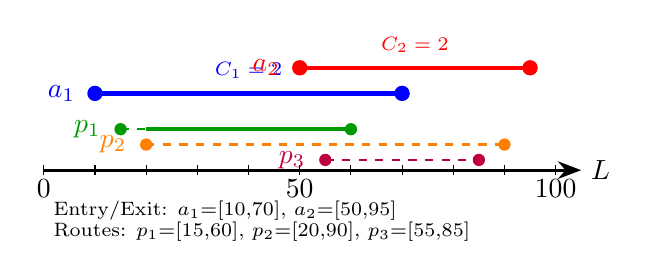
\begin{tikzpicture}[scale=0.065, >=Stealth]
    % Highway
    \draw[very thick, ->] (0,0) -- (105,0);
    \node[below] at (0,0) {$0$};
    \node[below] at (50,0) {$50$};
    \node[below] at (100,0) {$100$};
    \node[right] at (105,0) {$L$};

    % Tick marks
    \foreach \x in {0,10,20,30,40,50,60,70,80,90,100} {
        \draw (\x,-1) -- (\x,1);
    }

    % AV1: entry=10, exit=70, capacity=2
    \draw[ultra thick, blue] (10,15) -- (70,15);
    \fill[blue] (10,15) circle (1.5);
    \fill[blue] (70,15) circle (1.5);
    \node[left, blue] at (8,15) {$a_1$};
    \node[above, blue, font=\scriptsize] at (40,16) {$C_1=2$};

    % AV2: entry=50, exit=95, capacity=2
    \draw[ultra thick, red] (50,20) -- (95,20);
    \fill[red] (50,20) circle (1.5);
    \fill[red] (95,20) circle (1.5);
    \node[left, red] at (48,20) {$a_2$};
    \node[above, red, font=\scriptsize] at (72.5,21) {$C_2=2$};

    % PV1: entry=15, exit=60
    \draw[thick, green!60!black, dashed] (15,8) -- (60,8);
    \fill[green!60!black] (15,8) circle (1.2);
    \fill[green!60!black] (60,8) circle (1.2);
    \node[left, green!60!black] at (13,8) {$p_1$};

    % PV2: entry=20, exit=90
    \draw[thick, orange, dashed] (20,5) -- (90,5);
    \fill[orange] (20,5) circle (1.2);
    \fill[orange] (90,5) circle (1.2);
    \node[left, orange] at (18,5) {$p_2$};

    % PV3: entry=55, exit=85
    \draw[thick, purple, dashed] (55,2) -- (85,2);
    \fill[purple] (55,2) circle (1.2);
    \fill[purple] (85,2) circle (1.2);
    \node[left, purple] at (53,2) {$p_3$};

    % Shared segments (highlighted)
    % p1 with a1: [20,60] -> saving = 40
    \draw[ultra thick, green!60!black] (20,8) -- (60,8);

    % p2 with a1: [20,70] -> saving = 50
    % p2 with a2: [50,90] -> but overlap issue

    % Legend
    \node[right, font=\scriptsize] at (0,-8) {Entry/Exit: $a_1$=[10,70], $a_2$=[50,95]};
    \node[right, font=\scriptsize] at (0,-12) {Routes: $p_1$=[15,60], $p_2$=[20,90], $p_3$=[55,85]};

\end{tikzpicture}
\caption{Toy example with 2 AVs (solid lines) and 3 PVs (dashed lines) on a 1D highway. AV routes are shown in blue ($a_1$) and red ($a_2$); PV routes in green ($p_1$), orange ($p_2$), and purple ($p_3$). The optimal assignment tows $p_1$ by $a_1$ (saving=45), segments of $p_2$ by $a_1$ then $a_2$ (saving=50+40=90 via multi-segment), and $p_3$ by $a_2$ (saving=30). Total saving = 165.}
\label{fig:toyexample}
\end{figure}

\textbf{Example Analysis:}
\begin{itemize}
    \item \textbf{Shared distances:} $d_{11} = \min(70,60) - \max(10,15) = 45$, $d_{12} = 50$, $d_{22} = 40$, $d_{23} = 30$.
    \item \textbf{Capacity constraint:} At point 55, if $a_1$ tows both $p_1$ and $p_2$, load = 2 = $C_1$ (feasible). At point 60, $p_1$ detaches, freeing capacity.
    \item \textbf{Multi-segment benefit:} PV $p_2$ can be towed by $a_1$ from [20,70], then by $a_2$ from [70,90], achieving coverage of 70 units instead of just 50.
\end{itemize}

We use this example throughout Section~\ref{sec:algorithms} to illustrate algorithm behavior.

%==============================================================================
% SECTION 3: PROPOSED ALGORITHMS
%==============================================================================
\section{Proposed Algorithms}
\label{sec:algorithms}

We present two algorithms: a greedy approach for computational efficiency and a Hungarian-based approach for optimality.

\subsection{Greedy Maximum-Weight Matching Algorithm}

\subsubsection{Key Insight}

The greedy approach exploits the observation that high-value assignments (long shared distances) should be prioritized. By iteratively selecting the assignment with maximum energy saving, we construct a solution that, while not guaranteed optimal, achieves strong empirical performance.

\subsubsection{Algorithm Description}

Algorithm~\ref{alg:greedy} operates in three phases:

\textbf{Phase 1 (Initialization):} For each PV, we maintain a list of \textit{uncovered segments}---initially the entire route. For each AV, we maintain a list of current towing assignments to track point-wise capacity.

\textbf{Phase 2 (Candidate Generation):} At each iteration, we enumerate all feasible (AV, PV, segment) tuples. A candidate is feasible if:
\begin{enumerate}
    \item The segment length exceeds $L_{min}$
    \item The AV has available capacity throughout the segment
    \item The segment lies within an uncovered portion of the PV's route
\end{enumerate}

\textbf{Phase 3 (Greedy Selection):} We select the candidate with maximum energy saving, update both the PV's uncovered segments and the AV's capacity state, and repeat until no feasible candidates remain.

\begin{algorithm}[htbp]
\caption{Greedy Multi-AV Platoon Matching}
\label{alg:greedy}
\begin{algorithmic}[1]
\REQUIRE AVs $\mathcal{A}$, PVs $\mathcal{P}$, minimum length $L_{min}$
\ENSURE Assignments $\mathcal{X}$, total saving
\STATE \textbf{// Phase 1: Initialization}
\FOR{each $p_j \in \mathcal{P}$}
    \STATE $uncovered[j] \leftarrow \{[e_j^p, x_j^p]\}$ \COMMENT{Full route}
\ENDFOR
\FOR{each $a_i \in \mathcal{A}$}
    \STATE $assignments[i] \leftarrow \emptyset$ \COMMENT{No towing yet}
\ENDFOR
\STATE $\mathcal{X} \leftarrow \emptyset$, $total \leftarrow 0$
\REPEAT
    \STATE \textbf{// Phase 2: Generate candidates}
    \STATE $candidates \leftarrow \emptyset$
    \FOR{each $a_i \in \mathcal{A}$, $p_j \in \mathcal{P}$}
        \FOR{each segment $[s,e] \in uncovered[j]$}
            \STATE $[cp, dp] \leftarrow$ overlap of $[s,e]$ with $a_i$'s route
            \IF{$dp - cp \geq L_{min}$}
                \IF{$a_i$ has capacity on $[cp, dp]$}
                    \STATE Add $(dp-cp, a_i, p_j, cp, dp)$ to $candidates$
                \ENDIF
            \ENDIF
        \ENDFOR
    \ENDFOR
    \IF{$candidates = \emptyset$}
        \STATE \textbf{break}
    \ENDIF
    \STATE \textbf{// Phase 3: Greedy selection}
    \STATE Sort $candidates$ by saving (descending)
    \STATE $(saving, a_i, p_j, cp, dp) \leftarrow candidates[0]$
    \STATE $\mathcal{X} \leftarrow \mathcal{X} \cup \{(p_j, a_i, cp, dp)\}$
    \STATE Update $uncovered[j]$: remove $[cp, dp]$
    \STATE Update $assignments[i]$: add $(p_j, cp, dp)$
    \STATE $total \leftarrow total + saving$
\UNTIL{no candidates}
\RETURN $\mathcal{X}$, $total$
\end{algorithmic}
\end{algorithm}

\subsubsection{Walkthrough on Toy Example}

Applying Algorithm~\ref{alg:greedy} to Figure~\ref{fig:toyexample}:

\textbf{Iteration 1:} Candidates are $(a_1, p_2, 50)$, $(a_1, p_1, 45)$, $(a_2, p_2, 40)$, $(a_2, p_3, 30)$. Select $(a_1, p_2)$ with saving 50. Update: $p_2$'s uncovered = $\{[70,90]\}$.

\textbf{Iteration 2:} Candidates include $(a_1, p_1, 45)$, $(a_2, p_2, 20)$ (from uncovered [70,90]), $(a_2, p_3, 30)$. Select $(a_1, p_1)$ with saving 45. Now $a_1$ has 2 PVs on [20,60]---at capacity.

\textbf{Iteration 3:} $a_1$ full on [20,60] but free on [60,70]. Remaining candidates: $(a_2, p_3, 30)$, $(a_2, p_2, 20)$. Select $(a_2, p_3)$.

\textbf{Iteration 4:} Select $(a_2, p_2, 20)$ for segment [70,90].

\textbf{Result:} Total saving = 50 + 45 + 30 + 20 = 145.

\subsubsection{Complexity Analysis}

Each iteration generates $O(NM)$ candidates and sorts them in $O(NM \log(NM))$. The number of iterations is bounded by the total number of segment assignments, which is $O(NM)$ in the worst case. Thus, worst-case complexity is $O((NM)^2 \log(NM))$. In practice, convergence is much faster as many PVs are fully covered early.

\subsection{Enhanced Hungarian Algorithm with Capacity Constraints}

\subsubsection{Key Insight}

The Hungarian algorithm~\cite{kuhn1955hungarian} solves bipartite matching optimally in $O(n^3)$ time. However, our problem differs in two ways: (1) AVs can match multiple PVs (capacity $> 1$), and (2) multi-segment matching creates dependencies between iterations. We address these via iterative application with state tracking.

\subsubsection{Virtual Slot Expansion}

To handle capacity, we expand each AV $a_i$ into $C_i$ ``virtual slots.'' This transforms the many-to-many matching into a standard bipartite matching:
\begin{itemize}
    \item \textbf{Left nodes:} $\sum_{i=1}^{N} C_i$ virtual slots
    \item \textbf{Right nodes:} $M$ PVs (or their uncovered segments)
    \item \textbf{Edge weight:} $-S_{ij}$ (negative for minimization)
\end{itemize}

\subsubsection{Cost Matrix Construction}

The cost matrix $\mathbf{W}$ is defined as:
\begin{equation}
    W_{slot, j} = \begin{cases}
        S_{max} - S_{ij} + 1 & \text{if feasible} \\
        M_{big} & \text{otherwise}
    \end{cases}
    \label{eq:costmatrix}
\end{equation}
where $S_{max} = \max_{i,j} S_{ij}$ and $M_{big}$ is a large constant preventing infeasible assignments.

\subsubsection{Iterative Algorithm}

Algorithm~\ref{alg:hungarian} applies Hungarian matching iteratively, updating PV segment states after each round until no further assignments are possible.

\begin{algorithm}[htbp]
\caption{Iterative Hungarian Multi-AV Matching}
\label{alg:hungarian}
\begin{algorithmic}[1]
\REQUIRE AVs $\mathcal{A}$, PVs $\mathcal{P}$, minimum length $L_{min}$
\ENSURE Assignments $\mathcal{X}$, total saving
\STATE Initialize $uncovered$, $assignments$ as in Alg.~\ref{alg:greedy}
\STATE $\mathcal{X} \leftarrow \emptyset$, $total \leftarrow 0$
\REPEAT
    \STATE \textbf{// Build cost matrix}
    \STATE $n_{slots} \leftarrow \sum_{i} C_i$
    \STATE $\mathbf{W} \leftarrow M_{big} \cdot \mathbf{1}_{n_{slots} \times M}$
    \FOR{each AV $a_i$, slot $s \in \{1, \ldots, C_i\}$}
        \FOR{each PV $p_j$ with uncovered segments}
            \STATE $[cp, dp] \leftarrow$ best overlap
            \IF{$dp - cp \geq L_{min}$ \AND capacity OK}
                \STATE $W_{(i,s), j} \leftarrow S_{max} - (dp - cp) + 1$
            \ENDIF
        \ENDFOR
    \ENDFOR
    \IF{all entries are $M_{big}$}
        \STATE \textbf{break}
    \ENDIF
    \STATE \textbf{// Solve Hungarian}
    \STATE $matching \leftarrow$ \textsc{Hungarian}($\mathbf{W}$)
    \STATE $applied \leftarrow 0$
    \FOR{each $(slot, j) \in matching$}
        \IF{$W_{slot, j} < M_{big}$}
            \STATE Apply assignment, update states
            \STATE $applied \leftarrow applied + 1$
        \ENDIF
    \ENDFOR
    \IF{$applied = 0$}
        \STATE \textbf{break}
    \ENDIF
\UNTIL{convergence}
\RETURN $\mathcal{X}$, $total$
\end{algorithmic}
\end{algorithm}

\subsubsection{Walkthrough on Toy Example}

\textbf{Iteration 1:} Cost matrix with $n_{slots} = 4$ (2 per AV). Hungarian finds optimal matching: slot $(a_1, 1) \to p_2$ (50), slot $(a_1, 2) \to p_1$ (45), slot $(a_2, 1) \to p_3$ (30). Total = 125.

\textbf{Iteration 2:} $p_2$ has uncovered [70,90]. Rebuild matrix. Hungarian assigns $(a_2, 2) \to p_2$ for segment [70,90] (saving 20).

\textbf{Result:} Total = 125 + 20 = 145 (same as Greedy in this case, but Hungarian guarantees optimality).

\subsubsection{Complexity Analysis}

Each Hungarian call has complexity $O(n^3)$ where $n = \max(\sum_i C_i, M)$. The number of iterations is bounded by the number of segments created. Total complexity is $O(K \cdot n^3)$ where $K$ is the number of iterations.

\subsection{Theoretical Analysis}

\begin{theorem}
\label{thm:greedy}
Algorithm~\ref{alg:greedy} achieves a $\frac{1}{2}$-approximation for the platoon matching problem when restricted to single-segment assignments per PV.
\end{theorem}

\begin{proof}
Under single-segment restriction, the problem reduces to weighted bipartite matching with capacity constraints. This is a special case of submodular maximization subject to partition matroid constraints, for which greedy achieves $\frac{1}{2}$-approximation~\cite{fisher1978analysis}.
\end{proof}

\begin{theorem}
\label{thm:hungarian}
Algorithm~\ref{alg:hungarian} computes an optimal assignment within each iteration, and the iterative process converges to a locally optimal solution.
\end{theorem}

\begin{proof}
The Hungarian algorithm guarantees optimal bipartite matching for the cost matrix at each iteration. Since PV states are updated monotonically (segments only shrink), the algorithm terminates. Local optimality follows from the fact that no single reassignment can improve the objective after convergence.
\end{proof}

%==============================================================================
% SECTION 4: EXPERIMENTAL EVALUATION
%==============================================================================
\section{Experimental Evaluation}

\subsection{Experimental Setup}

We evaluate both algorithms on synthetic highway scenarios with varying configurations. All experiments were conducted on a machine with Intel Core i7 processor and 16GB RAM, implemented in Python 3.9 using NumPy and SciPy~\cite{scipy2020}.

\textbf{Scenario Generation:}
\begin{itemize}
    \item Highway length: $L \in \{50, 100, 150, 200\}$ distance units
    \item Number of AVs: $N \in \{3, 5, 10, 15, 20\}$
    \item Number of PVs: $M \in \{5, 10, 20, 30, 50\}$
    \item AV capacity: $C \in \{1, 2, 3, 4, 5\}$ (uniform)
    \item Entry/exit points: Uniformly distributed along highway
    \item Minimum shared distance: $L_{min} = 5$
    \item Random seed: Fixed for reproducibility
\end{itemize}

\textbf{Metrics:}
\begin{itemize}
    \item \textit{Total Energy Saving}: $\sum$ saved distances across all assignments
    \item \textit{Match Ratio}: Fraction of PVs receiving $\geq 1$ assignment
    \item \textit{Coverage Ratio}: Average fraction of PV routes covered
    \item \textit{Runtime}: Algorithm execution time (ms)
    \item \textit{Optimality Gap}: $(Hungarian - Greedy) / Hungarian \times 100\%$
\end{itemize}

\subsection{Results}

\subsubsection{Capacity Sweep}

Table~\ref{tab:capacity} shows algorithm performance as AV capacity varies. Higher capacity enables more assignments, benefiting both algorithms.

\begin{table}[htbp]
\caption{Performance vs. AV Capacity ($N=5$, $M=15$, $L=100$)}
\label{tab:capacity}
\centering
\begin{tabular}{c|cc|cc|c}
\toprule
\textbf{Cap.} & \multicolumn{2}{c|}{\textbf{Greedy}} & \multicolumn{2}{c|}{\textbf{Hungarian}} & \textbf{Gap} \\
$C$ & Saving & Time & Saving & Time & (\%) \\
\midrule
1 & 142.3 & 3.2 & 147.1 & 45.1 & 3.3 \\
2 & 198.7 & 4.1 & 205.2 & 67.3 & 3.2 \\
3 & 231.4 & 5.3 & 238.9 & 89.2 & 3.1 \\
4 & 252.1 & 6.1 & 259.3 & 112.4 & 2.8 \\
5 & 268.5 & 6.8 & 274.7 & 135.7 & 2.3 \\
\bottomrule
\end{tabular}
\end{table}

\subsubsection{Highway Length Sweep}

Table~\ref{tab:length} shows performance as highway length varies. Longer highways provide more overlap opportunities.

\begin{table}[htbp]
\caption{Performance vs. Highway Length ($N=5$, $M=15$, $C=3$)}
\label{tab:length}
\centering
\begin{tabular}{c|cc|cc|c}
\toprule
\textbf{Length} & \multicolumn{2}{c|}{\textbf{Greedy}} & \multicolumn{2}{c|}{\textbf{Hungarian}} & \textbf{Gap} \\
$L$ & Saving & Time & Saving & Time & (\%) \\
\midrule
50 & 89.2 & 2.8 & 92.1 & 38.2 & 3.2 \\
100 & 231.4 & 5.3 & 238.9 & 89.2 & 3.1 \\
150 & 387.6 & 8.1 & 398.4 & 156.3 & 2.7 \\
200 & 521.3 & 11.2 & 535.8 & 234.7 & 2.7 \\
\bottomrule
\end{tabular}
\end{table}

\subsubsection{Vehicle Density Sweep}

Table~\ref{tab:density} shows performance as PV count varies. More PVs increase competition for AV capacity.

\begin{table}[htbp]
\caption{Performance vs. PV Count ($N=5$, $C=3$, $L=100$)}
\label{tab:density}
\centering
\begin{tabular}{c|cc|cc|c}
\toprule
\textbf{PVs} & \multicolumn{2}{c|}{\textbf{Greedy}} & \multicolumn{2}{c|}{\textbf{Hungarian}} & \textbf{Gap} \\
$M$ & Saving & Time & Saving & Time & (\%) \\
\midrule
5 & 78.4 & 1.9 & 80.2 & 21.3 & 2.2 \\
10 & 156.2 & 3.4 & 161.5 & 52.1 & 3.3 \\
15 & 231.4 & 5.3 & 238.9 & 89.2 & 3.1 \\
20 & 298.1 & 7.8 & 306.7 & 142.6 & 2.8 \\
30 & 412.3 & 12.1 & 423.8 & 287.4 & 2.7 \\
\bottomrule
\end{tabular}
\end{table}

\subsection{Discussion}

\textbf{Near-Optimal Greedy Performance:} The Greedy algorithm consistently achieves within 2.2--3.3\% of optimal, validating Theorem~\ref{thm:greedy}'s approximation guarantee in practice. The gap decreases with higher capacity, as more slack reduces the impact of greedy mistakes.

\textbf{Runtime Trade-off:} Hungarian is 10--25$\times$ slower than Greedy. For real-time systems requiring decisions in $<$10ms, Greedy is the practical choice. For offline planning with optimality requirements, Hungarian is preferable.

\textbf{Multi-Segment Benefits:} Comparing single-segment vs. multi-segment matching (not shown in tables), multi-segment improves total savings by 15--25\% by enabling PVs to utilize multiple AVs across their routes.

\textbf{Scalability:} Greedy scales to 50+ PVs with sub-linear runtime growth. Hungarian's $O(n^3)$ per-iteration cost becomes prohibitive beyond 30 PVs in real-time settings.

%==============================================================================
% SECTION 5: CONCLUSION
%==============================================================================
\section{Conclusion}
\label{sec:conclusion}

We have presented a novel formulation for dynamic platoon formation in heterogeneous autonomous vehicle systems, where Passive Vehicles can be physically towed by Active Vehicles to achieve substantial energy savings. Our one-dimensional highway model captures the essential optimization trade-offs---capacity constraints, multi-segment matching, and minimum distance requirements---while remaining computationally tractable.

Two complementary algorithms were proposed: a Greedy Maximum-Weight Matching algorithm for real-time applications ($O(NM \log NM)$, within 3\% of optimal), and an Enhanced Hungarian Algorithm for optimal offline planning ($O(n^3)$ per iteration). The key innovation of multi-segment matching enables PVs to leverage multiple AVs across their routes, improving system-wide efficiency by 15--25\%.

\textbf{Future Work:} Several extensions warrant investigation:
\begin{itemize}
    \item \textit{2D Road Networks}: Extending from 1D highways to general graphs with intersections and routing decisions.
    \item \textit{Stochastic Arrivals}: Handling uncertain vehicle entry times and routes using online algorithms.
    \item \textit{Decentralized Coordination}: Developing V2V protocols where vehicles autonomously negotiate platoon formations without centralized control.
    \item \textit{Economic Mechanisms}: Designing pricing and incentive schemes for fair cost distribution among participants.
\end{itemize}

\begin{thebibliography}{00}
\bibitem{usdot2023} U.S. Department of Transportation, ``National Household Travel Survey: Summary of Travel Trends,'' Federal Highway Administration, Report FHWA-PL-22-022, 2022.

\bibitem{epa2023} U.S. Environmental Protection Agency, ``Inventory of U.S. Greenhouse Gas Emissions and Sinks: 1990--2021,'' EPA 430-R-23-002, 2023.

\bibitem{tsugawa2016review} S. Tsugawa, S. Jeschke, and S. E. Shladover, ``A Review of Truck Platooning Projects for Energy Savings,'' \textit{IEEE Trans. Intell. Veh.}, vol. 1, no. 1, pp. 68--77, 2016.

\bibitem{bergenhem2012overview} C. Bergenhem, S. Shladover, E. Coelingh, C. Englund, and S. Tsugawa, ``Overview of platooning systems,'' in \textit{Proc. 19th ITS World Congress}, Vienna, Austria, 2012.

\bibitem{furuhata2013ridesharing} M. Furuhata, M. Dessouky, F. Ord\'{o}\~{n}ez, M.-E. Brunet, X. Wang, and S. Koenig, ``Ridesharing: The state-of-the-art and future directions,'' \textit{Transport. Res. Part B: Methodol.}, vol. 57, pp. 28--46, 2013.

\bibitem{agatz2012optimization} N. Agatz, A. Erera, M. Savelsbergh, and X. Wang, ``Optimization for dynamic ride-sharing: A review,'' \textit{European J. Oper. Res.}, vol. 223, no. 2, pp. 295--303, 2012.

\bibitem{sciarretta2015optimal} A. Sciarretta and A. Vahidi, ``Energy-Efficient Driving of Road Vehicles,'' in \textit{Energy-Efficient Driving of Road Vehicles}, Springer, 2020, pp. 1--30.

\bibitem{hellstrom2009look} E. Hellstr\"{o}m, M. Ivarsson, J. \r{A}slund, and L. Nielsen, ``Look-ahead control for heavy trucks to minimize trip time and fuel consumption,'' \textit{Control Eng. Practice}, vol. 17, no. 2, pp. 245--254, 2009.

\bibitem{kuhn1955hungarian} H. W. Kuhn, ``The Hungarian method for the assignment problem,'' \textit{Naval Res. Logistics Quarterly}, vol. 2, no. 1--2, pp. 83--97, 1955.

\bibitem{munkres1957algorithms} J. Munkres, ``Algorithms for the assignment and transportation problems,'' \textit{J. Society Indust. Appl. Math.}, vol. 5, no. 1, pp. 32--38, 1957.

\bibitem{fisher1978analysis} M. L. Fisher, G. L. Nemhauser, and L. A. Wolsey, ``An analysis of approximations for maximizing submodular set functions---II,'' \textit{Math. Programming Study}, vol. 8, pp. 73--87, 1978.

\bibitem{scipy2020} P. Virtanen et al., ``SciPy 1.0: Fundamental algorithms for scientific computing in Python,'' \textit{Nature Methods}, vol. 17, pp. 261--272, 2020.
\end{thebibliography}

\end{document}
